\chapter{Megoldások telepítése, használata} \label{ch:usage}
A telepítés és a használat leírásának során feltételezem, hogy már fel van telepítve, és rendelkezésre áll a felhasználni kívánt QRadar, az ISIM, a TDI, valamint a megfelelő WebSphere. A fejlesztés és a tesztelés során felhasznált applikációk verziói a következők:

\begin{itemize}
	\item QRadar 7.2.8
	\item ISIM 6.0
	\item TDI 7.1.1
	\item WebSphere liberty 17.0.0.2
\end{itemize}



\section{TDI alapú integrációs modul}
A megoldás általam készített része egy wrapper, a hozzá tartozó segédosztályokkal, valamint egy TDI connector implementáció, ami a wrapperre épül. A wrapper önmagában is felhasználható más projektekben. A connector egy .jar formájában használható fel, amit a megfelelő TDI installáció \$INSTALL\_DIR\$/jars/connectors mappájába bemásolva használhatunk fel. 
\subsection{Dependenciák} \label{subsec:wrapdep}
A wrapper a HTTP hívások bonyolítására az Apache Wink\cite{wink} framework-öt használja, így ezen a library-n kívül szükség van ennek a dependenciáira is, mint például a J2EE bővítményekre.

A wrapper ezen kívül logolásra az SLF4J könyvtárat használja.\cite{slf4j}
%\footnote{\href{https://www.slf4j.org/}{SLF4J hivatalos oldala: https://www.slf4j.org/}}

Mivel a QRadar irányú kapcsolat SSL titkosított és ehhez 2048 bites kulcsot használ, valamint DHE kulcscserét, ezért bizonyos java verziók esetén hibák léphetnek fel az SSL Handshake folyamán
\footnote{\href{https://stackoverflow.com/questions/6851461/java-why-does-ssl-handshake-give-could-not-generate-dh-keypair-exception}{Megoldások 1.6-os Java esetén: https://stackoverflow.com/questions/6851461/java-why-does-ssl-handshake-give-could-not-generate-dh-keypair-exception}} \footnote{\href{https://developer.ibm.com/answers/questions/209245/ssl-exception-error-in-wesphere-application-server.html}{Megoldás 1.6-os Java és IBM WebSphere használata esetén: https://developer.ibm.com/answers/questions/209245/ssl-exception-error-in-wesphere-application-server.html}}.
Ajánlott a Java 1.7-es verzióját használni, amiben ezek már javítva vannak.
%milyen depek vannak -> JaxRS, java2ee, slf4j, apache wink.
\subsection{Telepítés}

\subsubsection{Fordítás}
Ha csak forráskód áll rendelkezésre, akkor szükséges a projekt lefordítása, és egy .jar fájlba csomagolása. A fordításhoz szükségesek a fent felsorolt dependenciák elérhetővé tétele, valamint kettő, a TDI által biztosított .jar fájl: \textit{miserver.jar} és \textit{miconfig.jar}. Ezek megtalálhatók a \textit{\$TDI\_INSTALL\$/jars/common} mappában. 
Az elkészült jar fájl tartalmazza a fordított .class fájlokat a megfelelő mappa struktúrában, valamint a gyökérkönyvtárban a \ref{subsec:connimpl}. fejezetben leírtaknak megfelelően elkészített tdi.xml-t.

\subsubsection{TDI oldali konfiguráció}
Ahhoz, hogy a TDI használni tudja a connector-t, az elkészített .jar fájlt be kell másolni a \textit{\$TDI\_INSTALL\$/jars/connectors} mappába, valamint a szükséges dependenciákat a \textit{\$TDI\_INSTALL\$/jars/3rdparty/others} mappába.
\subsection{Kommunikációs beállítások}

\subsubsection{SSL titkosítás beállítása}
Mivel a QRadar SSL titkosítást használ, amihez egy self-signed certificate-el rendelkezik, ezt a certificate-et hozzá kell adni a TDI által használt SSL keystore-okhoz. Erre a feladatra ajánlott a TDI-al együtt érkező Java installáció által biztosított Ikeyman\footnote{Elérési út: \textit{\$TDI\_install\_dir\$/jvm/jre/bin}} grafikus alkalmazás használata. A két keystore, amihez a kulcsokat hozzá kell adni a \textit{\$TDI\_install\_dir\$/testserver.jks} valamint a \textit{\$TDI\_install\_dir\$/serverapi/testadmin.jks}.\cite{qradarssl}

\subsubsection{Engedélyezett alkalmazás felvétele a QRadar oldalán }
A TDI connector - QRadar irányú autentikáció biztosításához szükséges egy QRadar API kulcs. Ezt a QRadar webes admin felületén, az \textit{Admin -> User Management -> Authorized Services} menüpont alatt található. Itt egy új rekord felvétele és felkonfigurálása után, az Authentication Token mezőben található token-t használva a connector felkonfigurálásához létrehozható a kapcsolat a REST API-val. 

Amennyiben biztonsági szempontból szükséges, beállítható, hogy a kulcsot használó applikációk milyen csoport tagsággal rendelkezzenek, valamint a hozzáférés elévülési ideje. A csoport tagság definiálja azt, hogy pontosan milyen típusú operációkhoz fog hozzáférni az alkalmazás, ezért fontos, hogy a connector által használt tokenhez tartozó csoport tudja írni és olvasni is a reference data-kat.

\subsection{Használat}
Az előzetes konfigurációs lépések elvégzése után a connector elérhető a TDI grafikus szerkesztőjén keresztül, és szabadon felhasználható assembly line-okban a többi, beépített connector-nak megfelelő módon. Egy ilyen felhasználásra mutat példát a \ref{subsec:conntest} fejezetben leírt példa. \cite{tditutorial}
\section{Websphere alapú alkalmazás}
\subsection{Dependenciák}
Az alkalmazás egy Java EE webalkalmazás, amely WebSphere alkalmazásszerverre lett tervezve, azon belül pedig a WebSphere Liberty változatára. Mivel csak ezen lett tesztelve, ezért más alkalmazásszerver nem támogatott, de apróbb változtatásokkal valószínűleg más szerveren is futtatható, de a leírásnak nem célja egy mindenre kiterjedő útmutatót adni. 

A teszteléshez 17.0.0.2-es Liberty installációt használtam, valamint fontos, hogy a Liberty szerver támogassa, és legyenek telepítve az alábbi beépülők: webProfile-7.0, localConnector-1.0, jsp-2.3, jca-1.7, concurrent-1.0, appSecurity-2.0, servlet-3.1, passwordUtilities-1.0, distributedMap-1.0.

%
%\begin{itemize}
%	\item webProfile-7.0
%	\item localConnector-1.0
%	\item jsp-2.3 - A weblapok megjelenítéséhez.
%	\item jca-1.7
%	\item concurrent-1.0 - A feladatok ütemezéséhez
%	\item appSecurity-2.0
%	\item servlet-3.1
%	\item passwordUtilities-1.0 - Az alkalmazás által használt technikai jelszavak kezeléséhez
%	\item distributedMap-1.0 - Az alkalmazás által használt DynaCache cache-elési módszerhez.
%\end{itemize}

Az ütemezéshez az alkalmazás a commonj \cite{commonj} könyvtárat használja, így ezt is elérhetővé kell tenni a szerver számára. 

Mivel ez az alkalmazás is az általam készített wrappert használja a QRadarral való kommunikációra, ezért a \ref{subsec:wrapdep}-ben leírtaknak megfelelően annak a dependenciáira is szükség van, nevezetesen az SLF4J könyvtárra, és az Apache Wink könyvtár megfelelő részeire.

Az alkalmazás működéséhez továbbá szükség van a megfelelő verziójú DB2-es Java driverre\footnote{A megfelelő verzió jelen esetben azt jelenti, hogy a felhasznált driverek az adott, felhasznált DB2 instanciának megfelelő driverek kell hogy legyenek} és licenszre, amiket az alkalmazás az ISIM adatbázisaihoz, valamint a saját adatbázisaihoz való kapcsolódásra használ. Ezeket egy library formájában fel kell venni a Liberty szerver definíciós XML-jébe, továbbá a megfelelő adatbázisokat a hozzájuk tartozó autentikációs adatokkal dataSource-ként.\cite{wsdatasource}

A fent említetteken kívül, valamint az általános konfigurációs értékeken kívül szükséges a szerverhez tartozó server.xml állományába felvenni / módosítani a következő konfigurációs értékeket:
\begin{itemize}
	\item distributedMap\cite{dynacache}: Az alkalmazás által használt DynaCache definíciója 
	\item managedScheduledExecutorService\cite{wsscheduler}: Az alkalmazás által használt ütemező definíciója
\end{itemize}

\subsection{Telepítés}
A dependenciák elérhetővé tétele, és a szerver megfelelő felkonfigurációja után az alkalmazás telepítésére két mód is rendelkezésre áll. Lehetőség van a lefordított alkalmazás csomagolt formában való elhelyezésére a Liberty által rendszeresen ellenőrzött \textit{dropins} mappában, vagy az alkalmazás konfigurációjában elhelyezni egy rekordot, ami az telepítendő applikáció elérési útját tartalmazza. \cite{wsdropin}

\begin{figure}[!h]
	\centering
	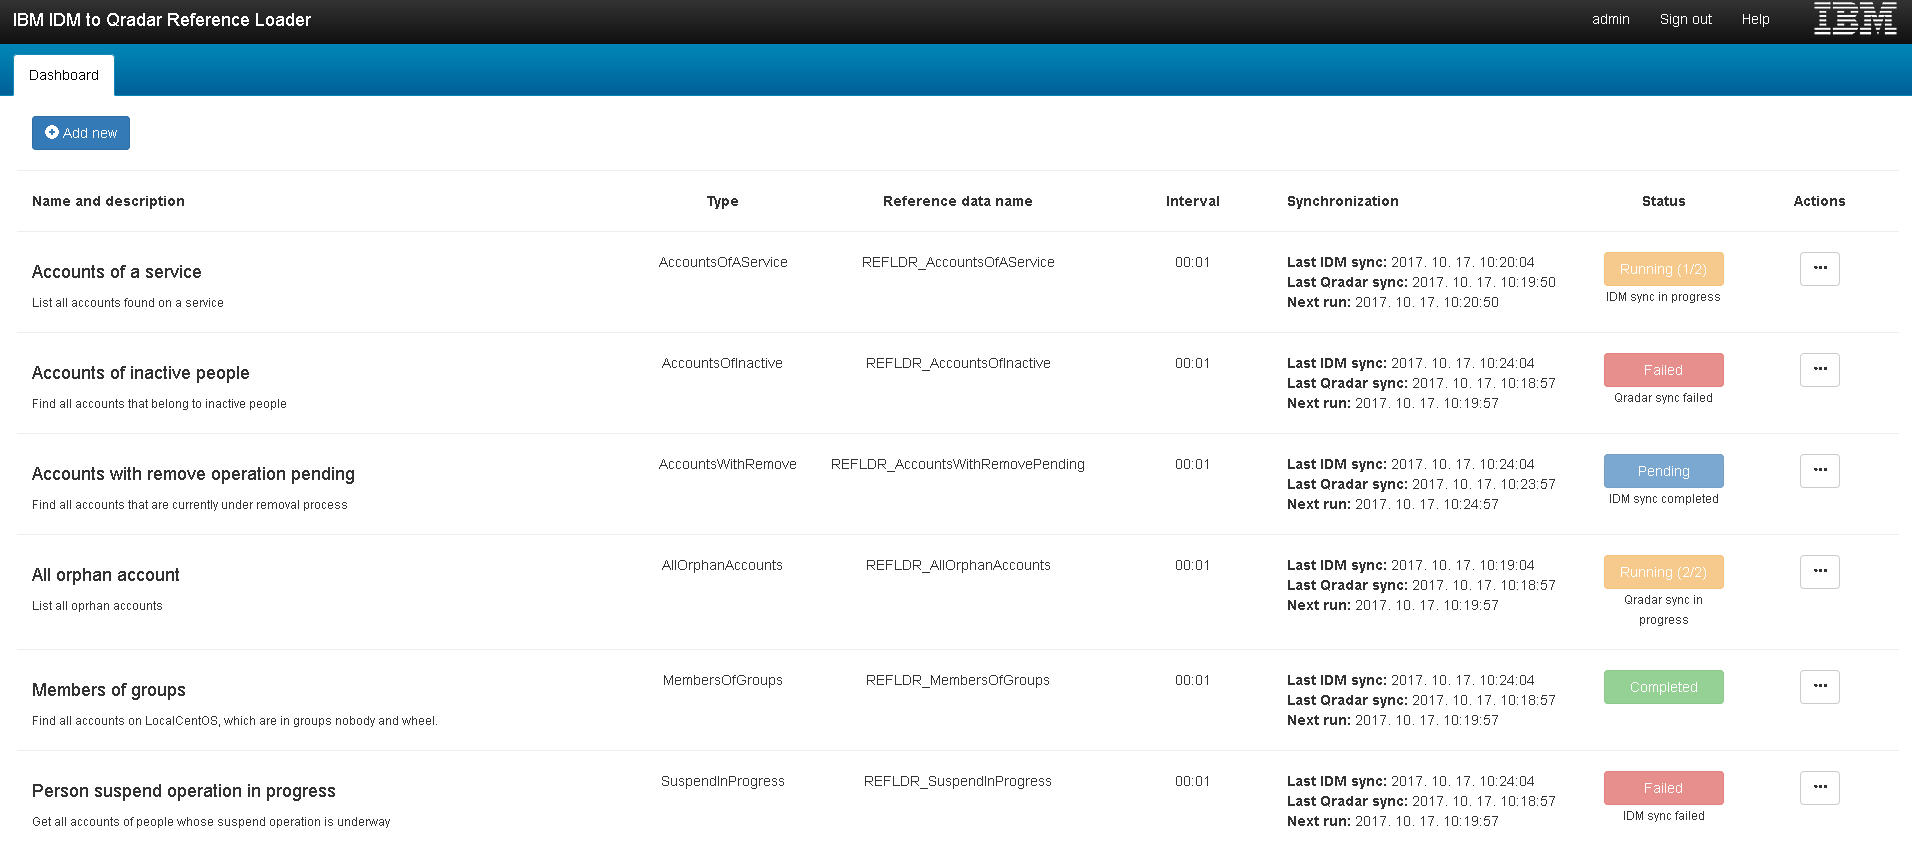
\includegraphics[width=0.8\linewidth]{figures/refloader_ui/all_states}
	\caption{A WebSphere alapú integrációs megoldás főképernyője, az összes lehetséges query állapottal.}
	\label{fig:allstates}
\end{figure}

\subsection{Használat}

Az alkalmazás egy Bootstrap alapú felhasználói felületről érhető el. A konfigurációban megadott bejelentkezési adatok segítségével belépve egy központi oldal fogad, amin láthatók a felkonfigurált lekérdezések, azok állapotai, valamint az ütemezési információik. A felületen megjelenített mezők jelentése a következő:



\begin{itemize}
	\item Name and description: A szinkronizációs feladat neve és leírása, amit annak felvételekor adhatunk meg.
	\item Type: A lekérdezés típusa
	\item Reference data name: A lekérdezés által kezelt reference data neve.
	\item Interval: A lekérdezés futtatási gyakorisága.
	\item Synchronization: Információk a lekérdezés ütemezésével kapcsolatban.
	\item Status: Információ a lekérdezés aktuális állapotáról.
	\item Actions: Lenyíló menü a lekérdezéssel kapcsolatos máveletek indítására.
\end{itemize}
\begin{figure}[!h]
	\centering
	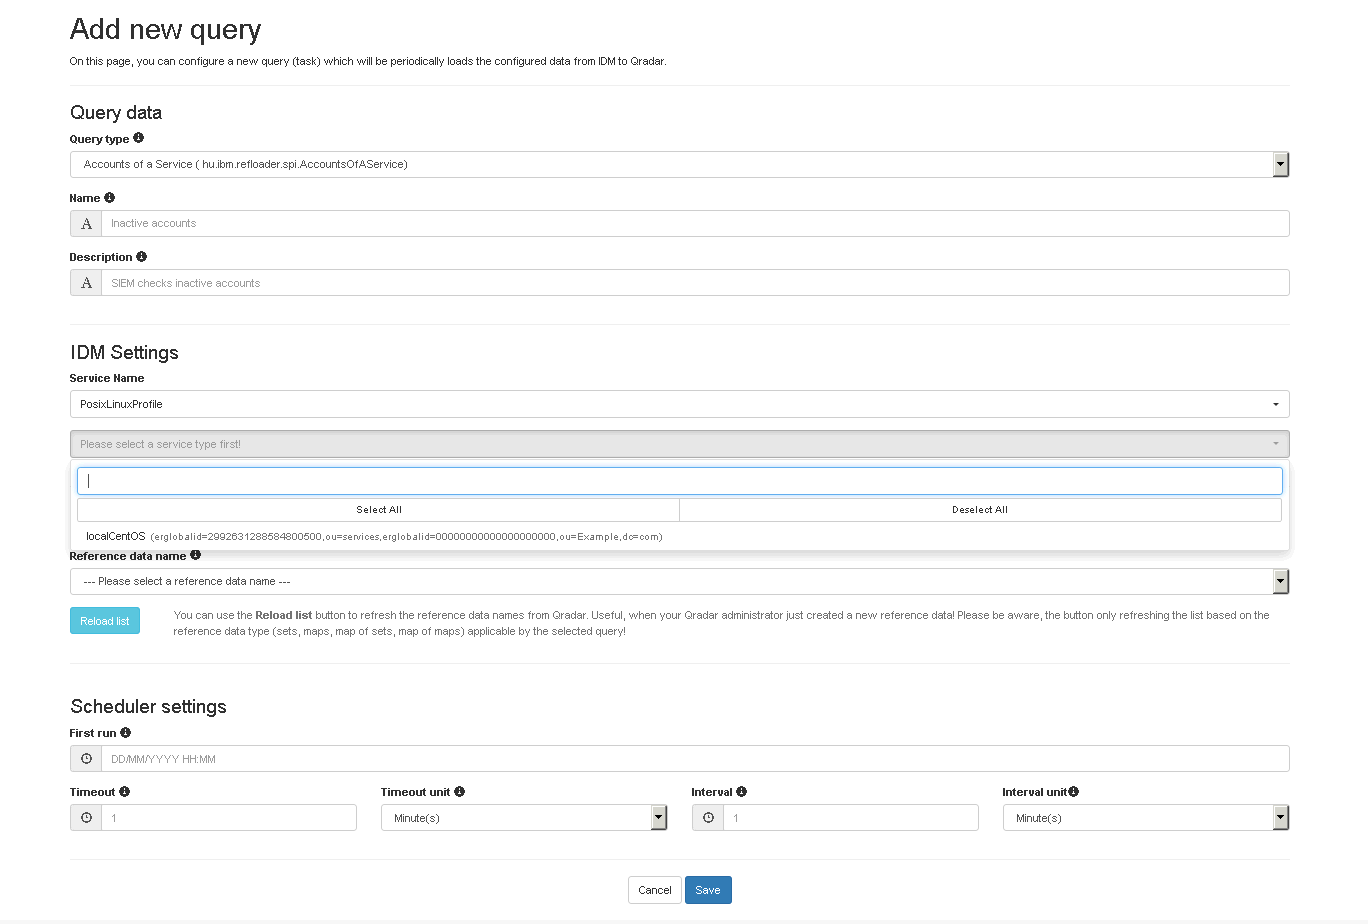
\includegraphics[width=0.8\linewidth]{figures/refloader_ui/add_new2}
	\caption{Az új query-k hozzáadását támogató felület}
	\label{fig:addnew}
\end{figure}

Egy felvett lekérdezés típuson 5 művelet típus hajtható végre, amik a következők:
\begin{itemize}
	\item Synchronize now: Az adott lekérdezést azonnal hozzáadja az ütemezési sorhoz, attól függetlenül, hogy milyen ütemezési paraméterekkel rendelkezik, és milyen állapotban van.
	\item Reload: Frissíti a lekérdezés állapotát és a hozzá kapcoslódó információkat a felületen.
	\item View content: Egy felugró ablakban megmutatja a feltöltött reference data állapotát, az alkalmazás által tárolt lokális állapot alapján.
	\item Preview: Az ISIM-ből lekérdezett adatokat mutatja olyan lekérdezéseknél, amelyek még nem töltötték fel az eredményeket a QRadarnak.
	\item Delete: Törli a lekérdezést.
\end{itemize}

Új query felvételéhez a bal felül található "Add query" gomb használható, ami egy új oldalra, a \ref{fig:addnew}. ábrán láthatóra irányít át. Ezen az oldalon megadhatjuk a query típusát, ami alapján az oldal kezelőfelülete megváltozik, és a query által használható paraméterek konfigurlását lehetővé tevő mezők lesznek elérhetők rajta. A mezők, ahol releváns, segítik a kitöltést, és felkínáljak a lehetséges inputokat. A felkonfiruált lekérdezést elmentve az bekerül az ütemezési sorba, és végrehajtódik, ha rá kerül a sor.



% \subsubsection{Fejlesztői útmutató} Legyen itt pár szó arról hogy hogyan lehet új query típusokat definiálni?
